% IEEE TCDS submission -- merged paper, single-thesis rewrite (v2).
%
% Merges two drafts by the same author: the two-routes comparison rescored at a
% converged budget with the body-model withdrawal made single-factor
% (wm_prior/tcds/paper.tex), and the teacher-withdrawal decomposition with the
% attachment axis, replacing regime and budget matching
% (world_model_zeroshot/paper/tcds/paper.tex). Numbers in Sections IV-A, IV-B
% and Tables I/II are audited against raw per-seed JSON by scratchpad
% merged_audit_tcds.py / audit_prose.py; Tables III-VI are carried over from
% the second draft and audited against its JSON by audit_merged_carried.py;
% Table VII (both decompositions at 100k) is filled from
% results_matched100k_elbow, results_coach100k_elbow (constant, abrupt) and
% results_coach100k_elbow_off2 (selfanchor with the swap on loop step t_w-2,
% the arm that reproduces the 12k table seed for seed) and audited by
% audit_w100k.py. The previous prose is kept as paper_v1_merged.tex.
\documentclass[journal]{IEEEtran}

\usepackage[hidelinks]{hyperref}
\usepackage{graphicx}
\usepackage{amsmath,amssymb}
\usepackage{booktabs}
\usepackage{url}

\renewcommand{\topfraction}{0.9}
\renewcommand{\dbltopfraction}{0.9}
\renewcommand{\textfraction}{0.07}
\renewcommand{\floatpagefraction}{0.85}
\renewcommand{\dblfloatpagefraction}{0.85}
\setcounter{topnumber}{3}
\setcounter{dbltopnumber}{3}
\setcounter{totalnumber}{5}

\newcommand{\ci}[3]{$#1\,[#2,\,#3]$}

\begin{document}

\title{What a Motor Prior Is Worth:\\
       A Frozen Body Model and a Teacher Compared to Convergence\\
       and Through Withdrawal}

\author{Mu-Hua~Wang%
  \thanks{The author is with the Department of Biomedical Engineering,
          National Yang Ming Chiao Tung University, Taipei, Taiwan
          (e-mail: may.be13@nycu.edu.tw).}}

\markboth{IEEE Transactions on Cognitive and Developmental Systems}%
         {Wang: What a Motor Prior Is Worth}

\maketitle

\begin{abstract}
Sensorimotor theory offers two accounts of what a learner brings to a motor
task: an internal forward model of the body, and guidance toward the correct
response. We instantiate both as priors for one soft actor-critic learner on
two MyoSuite musculoskeletal bodies, a frozen body model learned from
reward-free babbling and a frozen teacher acting through a distillation term,
with twelve matched seeds, an adversarial control for each route, and training
run until the arms stop moving. Three results follow. The body model helps
where the body is hard: its advantage over model-free learning is a transient
on a one-joint elbow and stable on a four-joint finger. Guidance is only as
good as its teacher: it keeps a small advantage on the elbow, whose teacher is
competent, while on the finger, whose teacher barely moves, a student held near
it ends worse than one given no aid. And withdrawing either prior costs no
dependence: with the learner's real-data signal held fixed, losing the body
model costs 22~mrad that has dissipated by convergence, and swapping the
teacher for a zero-information snapshot of the student shows that the immediate
drop after withdrawal is the deletion of a loss term, that no component grows
with attachment across seven durations and two coaching regimes, and that what
persists is the loss of the teacher's information. A fixed early endpoint
reverses the first two verdicts; matching the two priors' data budgets changes
neither.
\end{abstract}

\begin{IEEEkeywords}
Developmental robotics, sensorimotor learning, internal models, guidance
hypothesis, teacher--student distillation, reinforcement learning,
musculoskeletal control.
\end{IEEEkeywords}

\section{Introduction}

\IEEEPARstart{H}{umans} and animals acquire motor skills in a handful of
trials; deep reinforcement learning on muscle-actuated bodies can need hundreds
of millions of environment steps. Computational sensorimotor theory offers two
accounts of what a biological learner brings to a task that an agent trained
from scratch does not. One is an internal forward model of the body, predicting
the sensory consequences of motor commands \cite{wolpert1995,kawato1999} and
adapted in the intrinsic coordinates of joints and muscles \cite{shadmehr1994}.
The other is guidance: the guidance hypothesis
\cite{salmoni1984,schmidt1992,winstein1994} holds that augmented feedback
steers the learner toward the correct response while breeding a dependence on
it, so that the longer it is given the larger the fall when it is withdrawn.
Both are claims about a \emph{prior} in the developmental sense, something
present before task learning begins, and both can be instantiated for an
artificial learner and compared on equal terms.

We do that here. Under one soft actor-critic backbone on two MyoSuite bodies, a
one-joint elbow and a four-joint finger, we add either a frozen forward model
of the body, learned once from reward-free motor babbling and used for
short-horizon imagined rollouts, or a frozen teacher policy acting through a
distillation term. Each route is given the adversarial control the other has: a
random-initialised model in the same imagination machinery, a random-initialised
teacher in the same distillation loss. Every arm has twelve matched seeds, every
comparison is a paired contrast on the seed, and training runs until the arms
have stopped moving. We propose no algorithm. The claim is about what a motor
prior is worth, and it has three parts.

\emph{The body model helps where the body is hard.} Its advantage over
model-free learning is a transient of the first 12k steps on the elbow, not
detected at 100k, and a stable 40~mm on the finger, detected at every checkpoint
past 14k.

\emph{Guidance is only as good as its teacher.} On the elbow, whose teacher is
competent, the coached student keeps a small advantage at convergence. On the
finger, whose teacher is within 3.2~mm of doing nothing, a student held near it
ends 28~mm worse than one given no aid, and worse than one held near a random
teacher.

\emph{Withdrawing either prior costs no dependence.} Withdrawal as the
literature performs it changes two things at once. Purging the body model's
imagined buffer also doubles the learner's real-data gradient signal; with that
signal held fixed the loss costs $+22$~mrad on the elbow at 12k, where the
standard protocol detects nothing, and the cost has dissipated by 100k. Zeroing
a teacher's distillation weight deletes a loss term as well as the teacher's
information; replacing the teacher by a frozen snapshot of the student itself,
so that the term survives but carries nothing, shows that the immediate drop is
the loss term, that across seven attachment durations and two coaching regimes
no component grows with attachment, and that what persists at convergence is
about 8~mrad of genuinely lost teacher information.

Two checks close the case. Scored at 12k, as an earlier version of this study
scored it, the first two verdicts read the other way on both bodies: that
endpoint sat inside the only run of consecutive checkpoints at which the elbow
benefit was visible, and inside the only dip in which the finger benefit was
not. And the body model saw $3.3\times$ to $6.7\times$ more transitions than
the teacher; cut to the teacher's budget, its endpoint changes by $+1.6$~mrad
and $+2.8$~mm, neither detected. The runs, analysis scripts, and figures are
released with the paper.

\section{Background and Related Work}

\textbf{The guidance hypothesis.} Salmoni, Schmidt and Walter
\cite{salmoni1984} proposed that frequent or immediate augmented feedback guides
the learner to the correct response during acquisition while preventing the
processing that supports retention; when the feedback is removed, performance
falls. Schmidt and Bjork \cite{schmidt1992} generalised the account to practice
conditions at large, and Winstein, Pohl and Lewthwaite \cite{winstein1994}
showed the same pattern for physical guidance. Its best-known test
\cite{winstein1990} supports the retention limb more clearly than the
acquisition limb, and the reversal is weak across studies \cite{marschall2007}.
Two features matter here. It is a claim about \emph{dependence}: the learner is
worse after withdrawal than one who never had the guidance, or than one who had
less of it. And its mechanism is that guidance \emph{substitutes} for the
learner's own error detection and correction, so that the learner does not
practise them.

\textbf{Teacher--student learning in robotics.} Privileged learning
\cite{lee2020,kumar2021} trains a teacher with access to state the deployed
policy will not have, then distils it into a student through a behaviour
cloning loss on the student's own observations. In current legged and humanoid
pipelines \cite{rudin2022} the distillation stage may be the entire training of
the student, with no reward term; where a reward term is present the
distillation loss is auxiliary and is annealed or cut. In both cases the
post-withdrawal drop is used as a diagnostic, and the interpretation offered is
the guidance hypothesis' one, usually without naming it. We found no work in
reinforcement learning or robotics that runs a control for the loss term. A
policy initialised by behaviour cloning and then fine-tuned by off-policy
reinforcement often collapses at the transition, because the critic's errors on
out-of-distribution actions drive the actor away from the cloned behaviour
\cite{nair2020,uchendu2023,zhang2023}; Sec.~\ref{sec:replace} shows that this
transition, not the teacher, is what grows with attachment when guidance
replaces the learner's own signal.

\textbf{Model-based RL and body models.} World Models \cite{ha2018} and the
Dreamer series \cite{hafner2020,hafner2021,hafner2025} optimise a policy on
imagined rollouts while updating the model online; MBPO \cite{janner2019}
bounds compounding error with short rollouts branched from real data, the basis
for our Dyna step; PETS \cite{chua2018} and TD-MPC2 \cite{hansen2024} keep the
model learning throughout. Robot self-modelling \cite{bongard2006} infers a
body model from exploratory actions and goal babbling \cite{rolf2010} learns an
inverse model by directed exploration, where we use undirected babbling to
learn a forward model and freeze it. Plan2Explore \cite{sekar2020} and APV
\cite{seo2022} pretrain task-agnostic models in a reward-free phase; MOReL,
MOPO and COMBO \cite{kidambi2020,yu2020,yu2021} freeze a pretrained model and
optimise under it with pessimism, where we use a babble-learned model
optimistically and hand the arm the environment's analytic reward at imagined
states. Mainstream muscle RL is model-free
\cite{berg2023,chiappa2023,schumacher2023,wochner2022}; MuscleVAE
\cite{feng2023} and FreeMusco \cite{kim2025} learn world models for muscle
control but co-learn them during skill training. MyoSuite \cite{caggiano2022}
provides the bodies.

\section{Method}

\subsection{Bodies, task and backbone}
\texttt{myoElbowPose1D6M} is a one-degree-of-freedom elbow driven by six
muscles; error is a joint-angle error in milliradians (mrad).
\texttt{myoFingerReachRandom-v0} is a four-joint index finger driven by five
muscles reaching a three-dimensional fingertip target; error is a Euclidean
fingertip error in millimetres (mm). The two are never compared in magnitude.
The task is reach; episodes are 100 steps from a fixed start pose; training
draws from eight fixed targets; evaluation is greedy on twenty disjoint
held-out targets, so every number here is a generalisation measurement. One
soft actor-critic \cite{haarnoja2018} backbone is used in every condition: two
hidden layers of 128 units, update-to-data ratio~2, batch~128, 1{,}000 warm-up
steps, learning rate $3\times10^{-4}$, automatic entropy temperature.
Conditions differ only in what is added.

\subsection{The two priors}
The \emph{forward-model} route adds a body model $f_\theta(s,a)\mapsto s'$
trained once on task-agnostic, reward-free Ornstein--Uhlenbeck muscle
activations ($10^5$ transitions on the elbow, $2\times10^5$ on the finger), then
frozen, and used for short-horizon Dyna \cite{sutton1991} rollouts branched
from sampled real states; the environment's analytic reward is evaluated at the
imagined states, so every reading of this arm is scoped to a forward model
\emph{plus} a known reward function. Each update draws 64 real and 64 imagined
transitions where model-free arms draw 128 real.

The \emph{guidance} route adds a frozen teacher actor trained for 30k rewarded
steps on the same body. The student's actor loss is
\[
\mathcal{L}_\pi = q\,\mathcal{L}_{\mathrm{SAC}}
 + c\,\big\|\tanh\mu_{\mathrm{student}}(o) - \tanh\mu_{\mathrm{teacher}}(o)\big\|^2 ,
\]
on replayed observations $o$, with $c=1$ while the teacher is attached; the
critic trains on reward in every arm. In the \emph{additive} regime ($q=1$
always) the term supplements the student's own policy gradient, as concurrent
augmented feedback does; this is the coach used everywhere unless stated. In
the \emph{replacing} regime ($q=0$ while attached, $q=1$ from withdrawal) the
actor is moved only by the teacher until withdrawal, as physical guidance moves
the limb and as reward-free distillation \cite{rudin2022} does.

\subsection{Arms}
\textbf{Adversarial controls.} \texttt{randprior} replaces the babble-trained
model with a random-initialised frozen model in identical Dyna machinery;
\texttt{randcoach} replaces the trained teacher with a random-initialised one
distilled through the same loss at the same weight. \texttt{priorcoach} carries
both aids.

\textbf{Withdrawing the body model} at step 8000: \texttt{keep} never
withdraws; \texttt{soft} stops generating imagined transitions but leaves the
imagined buffer in place, so updates keep drawing 64 real and 64 stale
imagined; \texttt{purge} also empties the buffer, after which every batch is
128 real, the strict withdrawal of the original protocol, which removes
imagination and doubles distinct real transitions per update at once;
\texttt{matched} withdraws as \texttt{purge} does but draws 64 real
transitions and repeats them, holding distinct real transitions per update at
64. Real-data content is therefore 64 in \texttt{keep}, \texttt{soft} and
\texttt{matched} and 128 in \texttt{purge}, so only contrasts among the first
three are single-factor.

\textbf{Withdrawing the teacher} at step $t_w$: \texttt{none} (no teacher);
\texttt{constant} ($c=1$ throughout); \texttt{abrupt} ($c\to0$ at $t_w$, the
literature's withdrawal); \texttt{selfanchor} (at $t_w$ the teacher is replaced
by a frozen copy of the student's own actor, $c$ unchanged: the term survives
with the same weight and form but carries no external information);
\texttt{randanchor} (replaced by a freshly initialised actor); and, in the
replacing regime only, \texttt{gateon} ($q\to1$ at $t_w$ with the real teacher
kept). Three paired contrasts decompose the measured cost:
$\text{abrupt}-\text{constant}$ is losing the teacher \emph{and} the loss term,
$\text{selfanchor}-\text{constant}$ is losing the teacher only, and
$\text{abrupt}-\text{selfanchor}$ is losing the loss term only. The second is
where dependence would have to show up; the third is the confound. Snapshots
are taken of the student's actor on the student's observations, with any
observation normaliser frozen with them.

\subsection{Metrics and statistics}
\emph{Endpoint}: held-out error at the end of training. \emph{Dip}: error at
$t_w{+}1000$ minus error at $t_w$. \emph{Post-4k}: error 4{,}000 steps after
$t_w$, comparable across $t_w$. \emph{Attachment trend}: per-seed
ordinary-least-squares slope of a component against $t_w$, then a paired-$t$
interval across seeds, per 1{,}000 attached steps. The seed is the unit of
analysis and every arm has $n=12$ matched seeds; every comparison is a direct
paired contrast on the seed, never an inference from two separate verdicts;
intervals are paired-$t$ 95\% intervals with $\mathrm{df}=11$; an interval
excluding zero is called significant and marked~$^*$; a non-significant cell is
a failure to detect at this power, never evidence of equivalence.

\subsection{Reproduction}
Every arm of the converged grid reproduces the original study's 12k arm means
seed for seed at its 12k checkpoint, the withdrawal arms reproduce its kept,
soft-withdrawn and strict-withdrawn arms seed for seed, and the teacher-side
arms reproduce three published cells to the digit: myoElbow
$\text{abrupt}-\text{constant}$ endpoint \ci{+16.00}{+6.49}{+25.52}, myoElbow
body-model-versus-coach \ci{+10.89}{+2.52}{+19.26}, myoFinger
$\text{abrupt}-\text{constant}$ \ci{+46.37}{+22.88}{+69.87}. New arms are
measured on the same footing as the old ones.

\section{Results}
\begin{figure*}[!t]
\centering
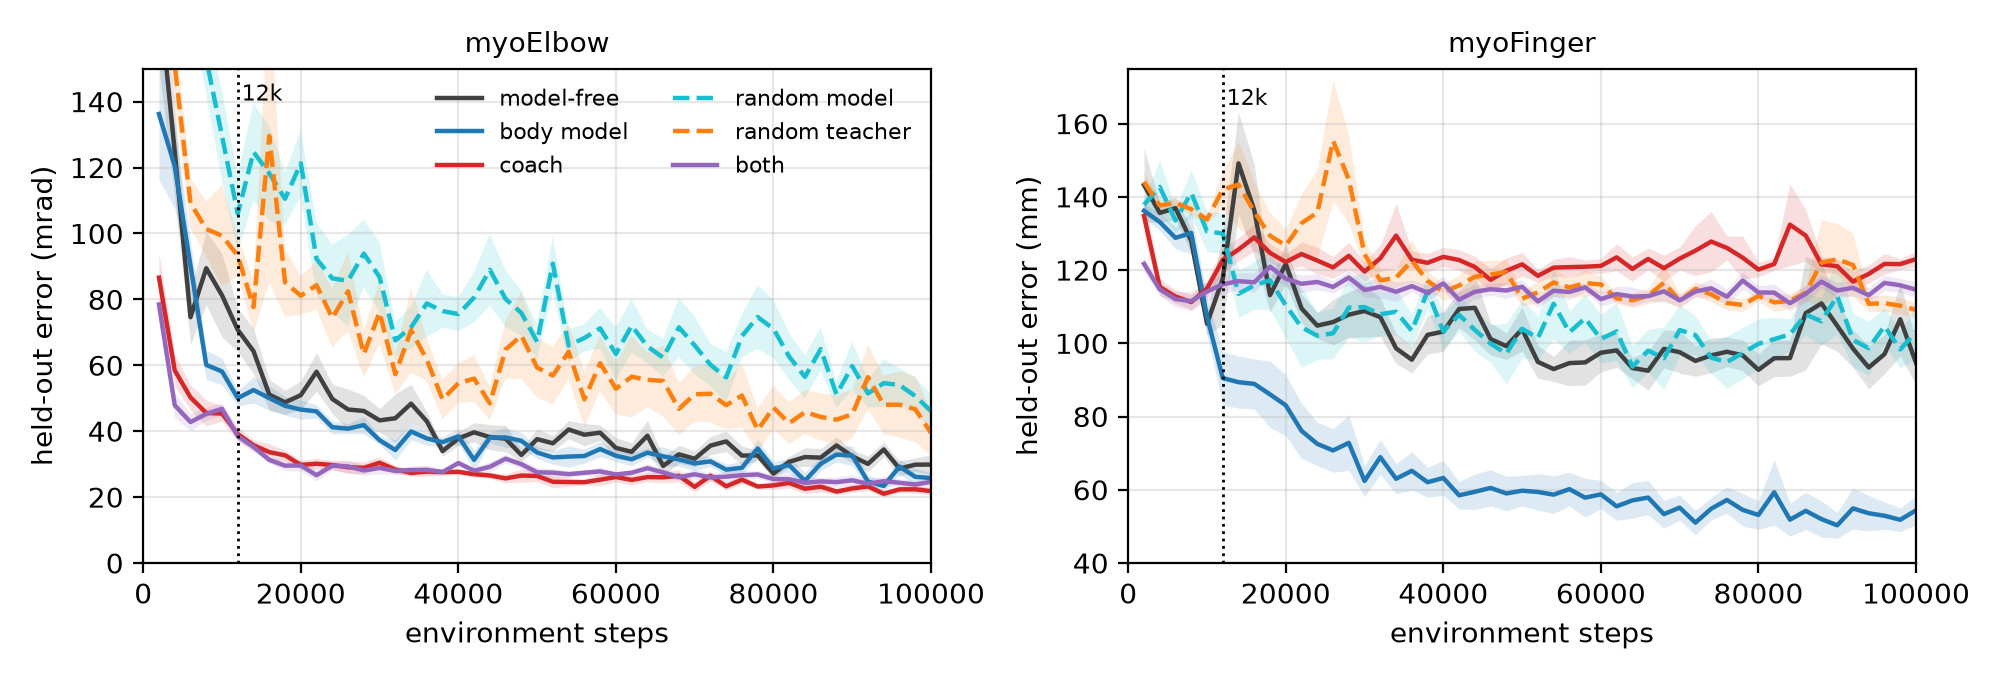
\includegraphics[width=0.96\textwidth]{figs/converged_curves.png}
\caption{Held-out error of the six core arms over 100{,}000 steps on myoElbow
(left, mrad; axis clipped at 150) and myoFinger (right, mm): mean across 12
seeds, band $\pm1$~SE, dashed lines the random controls. The dotted line marks
the 12k endpoint at which the original study scored every arm.}
\label{fig:conv}
\end{figure*}

\begin{table*}[!t]
\caption{The six core arms at a converged budget of 100{,}000 steps, held-out,
$n=12$. Arm means at 12k and 100k, then paired contrasts at 100k with 95\%
intervals; negative favours the first-named arm. The 12k checkpoints reproduce
the original study's arm means seed for seed (\texttt{randprior} was scored on
training targets there).}
\label{tab:conv}
\centering\small
\begin{tabular}{@{}lrrrr@{}}
\toprule
 & \multicolumn{2}{c}{myoElbow (mrad)} & \multicolumn{2}{c}{myoFinger (mm)} \\
 & 12k & 100k & 12k & 100k \\
\midrule
\texttt{blank}      & 70.73  & 29.87 & 117.60 & 94.66 \\
\texttt{prior}      & 50.02  & 25.78 & 90.50  & 54.37 \\
\texttt{randprior}  & 106.03 & 46.08 & 129.98 & 103.08 \\
\texttt{coach}      & 39.13  & 21.81 & 122.77 & 123.00 \\
\texttt{randcoach}  & 93.26  & 39.50 & 142.02 & 109.14 \\
\texttt{priorcoach} & 38.49  & 24.63 & 116.13 & 114.62 \\
\midrule
\texttt{coach}$-$\texttt{prior}     & $-10.89$ & $-3.97\ [-8.47, +0.53]$ & $+32.27$ & $\mathbf{+68.63}\ [+59.19, +78.07]$ \\
\texttt{prior}$-$\texttt{blank}     & $-20.72$ & $-4.09\ [-11.11, +2.94]$ & $-27.10$ & $\mathbf{-40.29}\ [-57.95, -22.64]$ \\
\texttt{coach}$-$\texttt{blank}     & $-31.61$ & $\mathbf{-8.06}\ [-15.83, -0.28]$ & $+5.17$ & $\mathbf{+28.33}\ [+16.11, +40.56]$ \\
\texttt{priorcoach}$-$\texttt{blank} & $-32.25$ & $-5.24\ [-12.93, +2.45]$ & $-1.47$ & $\mathbf{+19.96}\ [+5.74, +34.17]$ \\
\texttt{priorcoach}$-$\texttt{coach} & $-0.64$  & $+2.81\ [-1.02, +6.65]$ & $-6.64$ & $\mathbf{-8.38}\ [-15.57, -1.19]$ \\
\texttt{prior}$-$\texttt{randprior} & $-56.01$ & $\mathbf{-20.29}\ [-32.00, -8.59]$ & $-39.48$ & $\mathbf{-48.71}\ [-62.32, -35.09]$ \\
\texttt{coach}$-$\texttt{randcoach} & $-54.14$ & $\mathbf{-17.69}\ [-33.70, -1.68]$ & $-19.25$ & $\mathbf{+13.86}\ [+7.62, +20.09]$ \\
\bottomrule
\end{tabular}
\end{table*}

\begin{table}[!t]
\caption{Budget matching at 12k. Endpoint mean (seed s.d.) and paired
contrasts.}
\label{tab:budget}
\centering\scriptsize
\setlength{\tabcolsep}{2.5pt}
\resizebox{\columnwidth}{!}{%
\begin{tabular}{@{}lcc@{}}
\toprule
 & myoElbow (mrad) & myoFinger (mm)\\
\midrule
none                       & 70.73 (22.77) & 117.60 (43.03)\\
coach, 30k rewarded steps  & 39.13 (7.77)  & 122.77 (12.18)\\
prior, 30k babble          & 51.57 (8.73)  & 93.25 (22.02)\\
prior, full budget         & 50.02 (8.18)  & 90.50 (25.57)\\
\midrule
prior$_{30\mathrm{k}}$ $-$ prior$_{\mathrm{full}}$ & \ci{+1.55}{-0.87}{+3.97} & \ci{+2.75}{-12.77}{+18.27}\\
prior$_{\mathrm{full}}$ $-$ coach & \ci{+10.89}{+2.52}{+19.26}$^*$ & \ci{-32.27}{-48.05}{-16.49}$^*$\\
prior$_{30\mathrm{k}}$ $-$ coach & \ci{+12.44}{+3.27}{+21.61}$^*$ & \ci{-29.52}{-43.17}{-15.87}$^*$\\
\bottomrule
\end{tabular}}
\end{table}

\subsection{The body decides between the routes}
\label{sec:conv}
Table~\ref{tab:conv} and Fig.~\ref{fig:conv} score the six core arms at
100{,}000 steps. On myoElbow
every arm but the random-model control has stopped moving: over the last
20{,}000 steps \texttt{blank}, \texttt{prior} and \texttt{coach} change by
$+2.7$, $-2.9$ and $-1.7$~mrad against across-seed SDs of 11.3, 9.4 and 3.5;
\texttt{randprior} is still falling ($-25.0$, SD 29.6). The forward-model
route's advantage over model-free learning, $-20.72$~mrad $[-35.8,-5.6]$ at
12k, is \ci{-4.09}{-11.11}{+2.94} at 100k and is not detected; across fifty
checkpoints it is significant at seven: 8k, 10k and 12k, and four isolated later
ones with no two adjacent. The guidance route's advantage shrinks from
$-31.61$ $[-48.6,-14.6]$ to \ci{-8.06}{-15.83}{-0.28} but is still detected, at
43 of 50 checkpoints. The coach's lead over the body model, $-10.89$
$[-19.3,-2.5]$ at 12k, decays to \ci{-3.97}{-8.47}{+0.53} and is not detected
at the endpoint, though it is at 38 of 50 checkpoints including 96k; it does
not reverse on this body within the budget. The content of each aid matters:
the babble-trained model beats the random one by \ci{-20.29}{-32.00}{-8.59} and
the trained teacher beats the random one by \ci{-17.69}{-33.70}{-1.68}; the
random model is itself worse than model-free learning
(\ci{+16.21}{+6.82}{+25.59}), the random teacher not distinguishable from it
(\ci{+9.63}{-8.07}{+27.34}). Combining the aids adds nothing detectable:
\texttt{priorcoach} is \ci{-5.24}{-12.93}{+2.45} against model-free learning
and \ci{+2.81}{-1.02}{+6.65} against the coach alone.

On myoFinger the same budget moves the verdicts the other way. The body model's
advantage over model-free learning, not detected at 12k ($-27.10$
$[-66.3,+12.1]$), is \ci{-40.29}{-57.95}{-22.64} at 100k and is detected at
every checkpoint from 14k onward, 45 of 50 in all; the 12k endpoint sat in the
one dip in which it was not. The guidance route does not improve past 12k on
this body (122.77~mm at 12k, 123.00 at 100k), so the ordering of the two
routes, already reversed at 12k ($+32.27$ $[+16.5,+48.0]$ for
$\text{coach}-\text{prior}$), widens to \ci{+68.63}{+59.19}{+78.07} and holds at
every checkpoint from 12k on. From 40k on the constant-weight coach is
significantly worse than model-free learning at 27 of 31 checkpoints,
\ci{+28.33}{+16.11}{+40.56} at 100k. The finger teacher as captured sits within
3.2~mm of the no-op referent (Sec.~\ref{sec:limits}); a student held near it by
a constant pull is held near a policy that barely moves. The random-model
control holds (\ci{-48.71}{-62.32}{-35.09}, the random model not
distinguishable from model-free learning at \ci{+8.41}{-14.17}{+30.99}); the
random-teacher control reverses: at 12k the trained teacher beats the random one
by $-19.25$, at 100k the random one is better by \ci{+13.86}{+7.62}{+20.09},
and is itself worse than model-free learning (\ci{+14.48}{+0.74}{+28.21}).
Combining the aids inherits the coach's ceiling: \texttt{priorcoach} finishes
\ci{-8.38}{-15.57}{-1.19} better than the coach alone, \ci{+60.25}{+51.14}{+69.36}
worse than the body model alone and \ci{+19.96}{+5.74}{+34.17} worse than no aid.

The 12k endpoint was therefore not a neutral place to score. It overstated the
body model on the elbow, where the only run of checkpoints at which its benefit
was detectable was 8k to 12k, and understated it on the finger, where its
benefit was detectable everywhere except a dip that contained 12k. The coach's
ordering relative to the body model is body-dependent, and on both bodies the
direction it takes by 12k is the direction it keeps.

\textbf{Budget matching.}
\label{sec:budget}
The body model saw 3.3$\times$ (elbow) to 6.7$\times$ (finger) more transitions
than the teacher. We rebuilt the finger prior from exactly 30k babble
transitions with the same recipe and reused a 30k elbow prior from the original
budget sweep. Table~\ref{tab:budget} shows that cutting the budget changes the
endpoint by \ci{+1.55}{-0.87}{+3.97}~mrad and \ci{+2.75}{-12.77}{+18.27}~mm,
although the finger model's five-step prediction error rises from 14.3 to
25.1~mm; the finger reversal survives matching. Matching raw transition counts
is not matching information: the teacher's 30k steps are rewarded and on-task,
the prior's are not, and the prior arm holds the analytic reward at imagined
states.

\subsection{Withdrawing the body model costs a transient}
\label{sec:withdraw}
\begin{figure*}[!t]
\centering
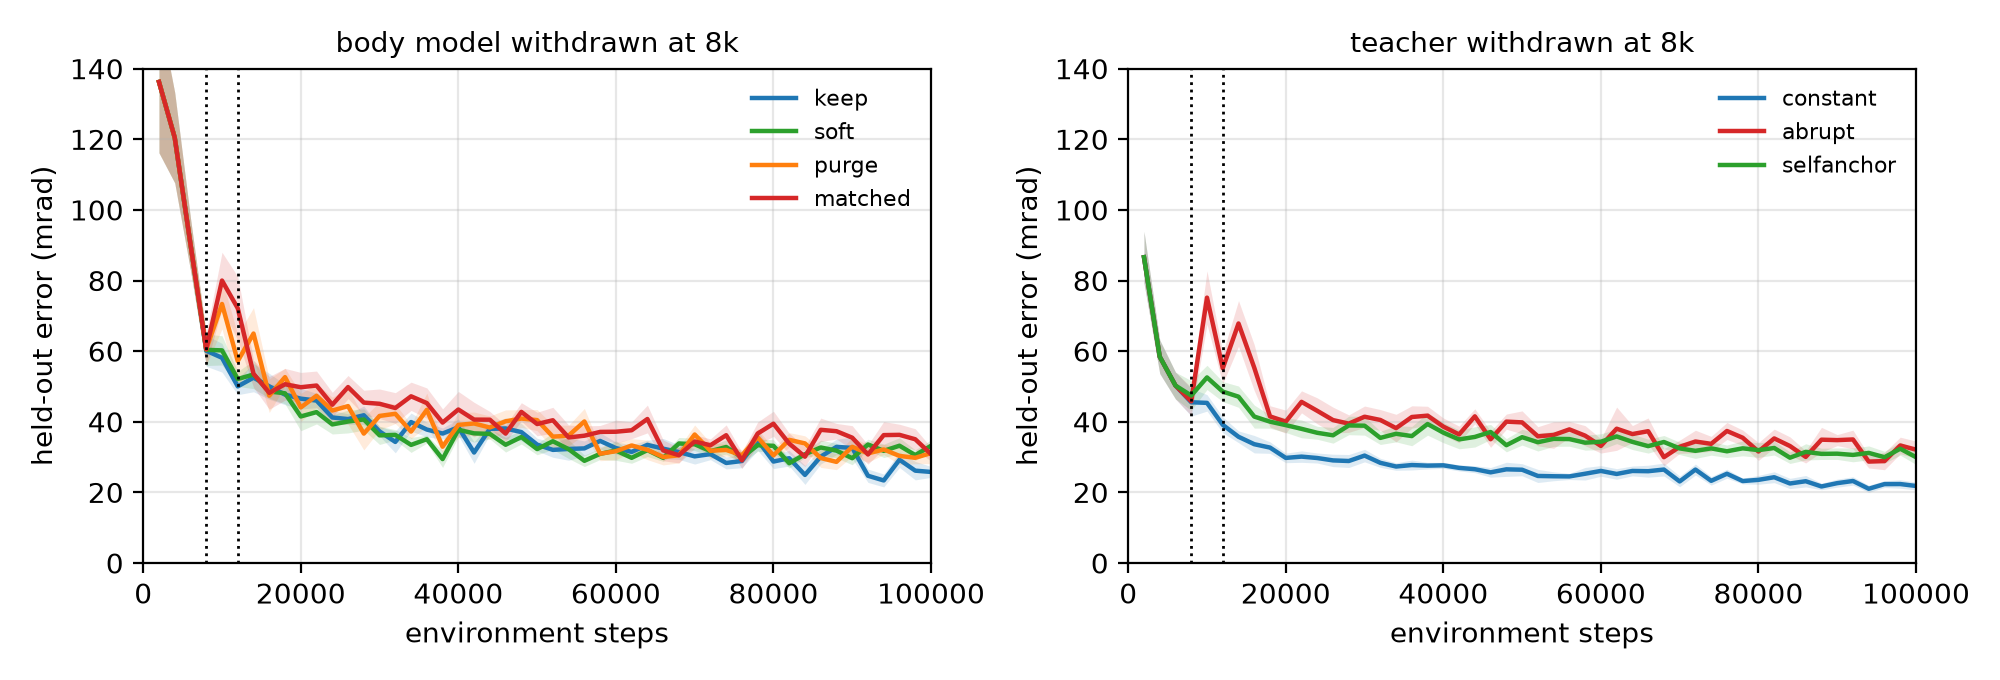
\includegraphics[width=0.96\textwidth]{figs/withdrawal100k_curves.png}
\caption{Both withdrawals on myoElbow run to 100{,}000 steps (mean across 12
seeds, band $\pm1$~SE; dotted lines at the withdrawal step 8000 and at 12k).
Left: the four body-model arms. Right: the three teacher arms. The body-model
arms converge on one another; the two withdrawn-teacher arms stay above
\texttt{constant}.}
\label{fig:w100k}
\end{figure*}

\begin{table*}[!t]
\caption{Withdrawal of the body model at step 8000, scored at 12000, held-out,
$n=12$. Means, then paired contrasts with 95\% intervals; positive means
withdrawal made the arm worse. $\dagger$: single-factor (real-data content equal
on both sides).}
\label{tab:withdraw}
\centering\small
\begin{tabular}{@{}lrr@{}}
\toprule
 & myoElbow (mrad) & myoFinger (mm) \\
\midrule
\texttt{keep}    & 50.02 & 90.50 \\
\texttt{soft}    & 52.11 & 88.11 \\
\texttt{purge}   & 57.19 & 104.69 \\
\texttt{matched} & 72.13 & 100.48 \\
\midrule
\texttt{purge}$-$\texttt{keep}            & $+7.17\ [-10.95, +25.29]$ & $+14.19\ [-0.95, +29.33]$ \\
\texttt{soft}$-$\texttt{keep}$^\dagger$    & $+2.09\ [-2.85, +7.04]$ & $-2.39\ [-13.74, +8.97]$ \\
\texttt{matched}$-$\texttt{keep}$^\dagger$ & $\mathbf{+22.11}\ [+4.94, +39.28]$ & $+9.97\ [-1.50, +21.45]$ \\
\texttt{soft}$-$\texttt{matched}$^\dagger$ & $\mathbf{-20.02}\ [-37.34, -2.70]$ & $-12.36\ [-24.84, +0.12]$ \\
\texttt{purge}$-$\texttt{matched}         & $-14.94\ [-44.62, +14.73]$ & $+4.22\ [-12.76, +21.19]$ \\
\bottomrule
\end{tabular}
\end{table*}
Table~\ref{tab:withdraw} gives the four arms at 12k. Measured as the original
protocol measured it, withdrawing the body model has no detectable cost on
myoElbow: $\text{purge}-\text{keep}$ is \ci{+7.17}{-10.95}{+25.29}. With
distinct real transitions per update held at 64, the same withdrawal is
significantly costly: $\text{matched}-\text{keep}$ is
\ci{+22.11}{+4.94}{+39.28}, and the change across the cut itself (8000 to
10000) is \ci{+21.47}{+4.54}{+38.40}. The two protocols reach different
verdicts because the strict withdrawal doubles the agent's real-data gradient
signal at the moment it loses the model, and that gain offsets part of the
loss; the direct contrast $\text{purge}-\text{matched}$ is
\ci{-14.94}{-44.62}{+14.73} and not significant, so we do not put a number on
the offset. The \texttt{soft} arm locates the cost: with real-data content
equal, keeping the stale imagined transitions rather than deleting them is
worth \ci{-20.02}{-37.34}{-2.70} ($\text{soft}-\text{matched}$), while keeping
them stale rather than fresh costs \ci{+2.09}{-2.85}{+7.04}, not detected. By
8000 steps what the frozen body model is worth on the elbow is carried by the
imagined transitions already in the buffer. On myoFinger neither protocol
detects a cost ($\text{purge}-\text{keep}$ \ci{+14.19}{-0.95}{+29.33};
$\text{matched}-\text{keep}$ \ci{+9.97}{-1.50}{+21.45}), so this is an elbow
result.

It is also a transient. Table~\ref{tab:w100k} and Fig.~\ref{fig:w100k} run the
same arms and seeds to 100{,}000 steps; their 12k checkpoints reproduce the 12k runs seed for seed.
By 100k the three withdrawn arms sit within 5--7~mrad of \texttt{keep} (25.78)
and within 2.4 of one another: $\text{matched}-\text{keep}$ is
\ci{+5.05}{-0.98}{+11.08}, no longer detected, and
$\text{soft}-\text{matched}$ is \ci{+2.35}{-4.42}{+9.11}. The one contrast
detected at 100k runs the other way from 12k: keeping the stale buffer is now
the worst of the four arms, $\text{soft}-\text{keep}$
\ci{+7.40}{+2.72}{+12.08}. What the matched control showed at 12k is a
statement about what the standard protocol misses in the window it scores, not
a persistent cost; on this body, after enough training, a learner that lost
its body model is close to one that kept it.

\subsection{Withdrawing the teacher costs no dependence}
\label{sec:decomp}

\begin{table}[!t]
\caption{Teacher withdrawal decomposed at $t_w=8000$, $n=12$; $^*$ marks an
interval excluding zero. Elbow in mrad, finger in mm.}
\label{tab:decomp}
\centering\footnotesize
\setlength{\tabcolsep}{3pt}
\begin{tabular}{@{}lcccc@{}}
\toprule
 & \multicolumn{2}{c}{myoElbow} & \multicolumn{2}{c}{myoFinger}\\
\cmidrule(lr){2-3}\cmidrule(lr){4-5}
Contrast & dip & endpoint & dip & endpoint\\
\midrule
abrupt $-$ constant (total)          & $+45.17^*$ & $+16.00^*$ & $+13.86^*$ & $+46.37^*$\\
selfanchor $-$ constant (teacher)    & $+4.95$    & $+9.42^*$  & $-0.27$    & $\mathbf{-11.29^*}$\\
abrupt $-$ selfanchor (loss term)    & $+40.22^*$ & $+6.59$    & $+14.13^*$ & $+57.66^*$\\
randanchor $-$ selfanchor            & $+47.44^*$ & $+20.66^*$ & $+20.13^*$ & $+17.20^*$\\
constant $-$ none                    & --         & $-31.61^*$ & --         & $+5.17$\\
\midrule
\multicolumn{5}{@{}l}{\footnotesize Seeds recovering pre-withdrawal error (of 12): elbow none 11, constant 7,}\\
\multicolumn{5}{@{}l}{\footnotesize abrupt 6, selfanchor 8, randanchor 5; finger 12, 6, 6, 12, 3.}\\
\bottomrule
\end{tabular}
\end{table}

\begin{table*}[!t]
\caption{Teacher-withdrawal components against attachment duration $t_w$.
Slope: per-seed OLS over $t_w$, paired-$t$ interval, per 1{,}000 attached steps.
Endpoint rows are not on equal footing across $t_w$.}
\label{tab:sweep}
\centering\small
\setlength{\tabcolsep}{5pt}
\begin{tabular}{@{}llccccccc l@{}}
\toprule
 & & 2k & 3k & 4k & 5k & 6k & 7k & 8k & slope\\
\midrule
\multicolumn{10}{@{}l}{\emph{myoElbow (mrad)}}\\
dip      & teacher   & $46.0^*$ & $22.0^*$ & $25.6^*$ & $1.5$ & $2.7$ & $7.8$ & $5.0$ & $\mathbf{-6.23}$ $[-7.79,\,-4.68]^*$\\
         & loss term & $13.6$ & $17.7^*$ & $37.9^*$ & $42.6$ & $77.9^*$ & $24.3^*$ & $40.2^*$ & $+4.76$ $[-0.13,\,+9.65]$\\
         & total     & $59.5^*$ & $39.7^*$ & $63.6^*$ & $44.1^*$ & $80.6^*$ & $32.1^*$ & $45.2^*$ & $-1.47$ $[-5.79,\,+2.84]$\\
post-4k  & teacher   & $25.1^*$ & $22.1^*$ & $8.2$ & $3.4$ & $4.2$ & $7.2$ & $9.4^*$ & $-2.88$ $[-5.86,\,+0.10]$\\
         & loss term & $9.0$ & $61.9^*$ & $34.7^*$ & $26.5^*$ & $36.2$ & $21.2^*$ & $6.6$ & $-3.11$ $[-8.69,\,+2.46]$\\
         & total     & $34.1^*$ & $84.0^*$ & $42.9^*$ & $29.9^*$ & $40.3^*$ & $28.4^*$ & $16.0^*$ & $\mathbf{-6.00}$ $[-10.60,\,-1.39]^*$\\
endpoint & teacher   & $27.9^*$ & $11.4^*$ & $5.6$ & $2.4$ & $6.4$ & $7.0$ & $9.4^*$ & $-2.26$ $[-4.84,\,+0.31]$\\
         & loss term & $-2.8$ & $17.9$ & $34.7^*$ & $23.8^*$ & $19.1$ & $22.4^*$ & $6.6$ & $+0.77$ $[-2.82,\,+4.36]$\\
\midrule
\multicolumn{10}{@{}l}{\emph{myoFinger (mm)}}\\
dip      & teacher   & $-0.6$ & $4.4$ & $7.0$ & $4.8$ & $0.4$ & $2.2$ & $-0.3$ & $-0.35$ $[-1.46,\,+0.75]$\\
         & loss term & $7.3$ & $4.6$ & $8.0^*$ & $10.0$ & $13.7^*$ & $20.7^*$ & $14.1^*$ & $\mathbf{+2.09}$ $[+0.46,\,+3.72]^*$\\
         & total     & $6.6$ & $8.9^*$ & $15.0^*$ & $14.8^*$ & $14.1^*$ & $22.8^*$ & $13.9^*$ & $\mathbf{+1.74}$ $[+0.25,\,+3.22]^*$\\
post-4k  & teacher   & $7.5^*$ & $3.9$ & $7.0^*$ & $4.0$ & $3.5$ & $-6.4^*$ & $-11.3^*$ & $\mathbf{-2.87}$ $[-4.27,\,-1.47]^*$\\
         & loss term & $14.7^*$ & $7.1$ & $14.3^*$ & $3.7$ & $-0.8$ & $30.4$ & $57.7^*$ & $\mathbf{+5.74}$ $[+1.49,\,+9.98]^*$\\
         & total     & $22.2^*$ & $10.9^*$ & $21.3^*$ & $7.7$ & $2.7$ & $24.1$ & $46.4^*$ & $+2.87$ $[-1.74,\,+7.47]$\\
endpoint & teacher   & $-3.3$ & $-4.8$ & $-10.0^*$ & $-10.5^*$ & $-9.9^*$ & $-9.9^*$ & $-11.3^*$ & $-1.21$ $[-2.52,\,+0.10]$\\
         & loss term & $2.6$ & $9.6$ & $-1.0$ & $21.5$ & $13.4$ & $55.1^*$ & $57.7^*$ & $\mathbf{+9.67}$ $[+5.54,\,+13.80]^*$\\
\bottomrule
\end{tabular}
\end{table*}

\begin{figure*}[!t]
\centering
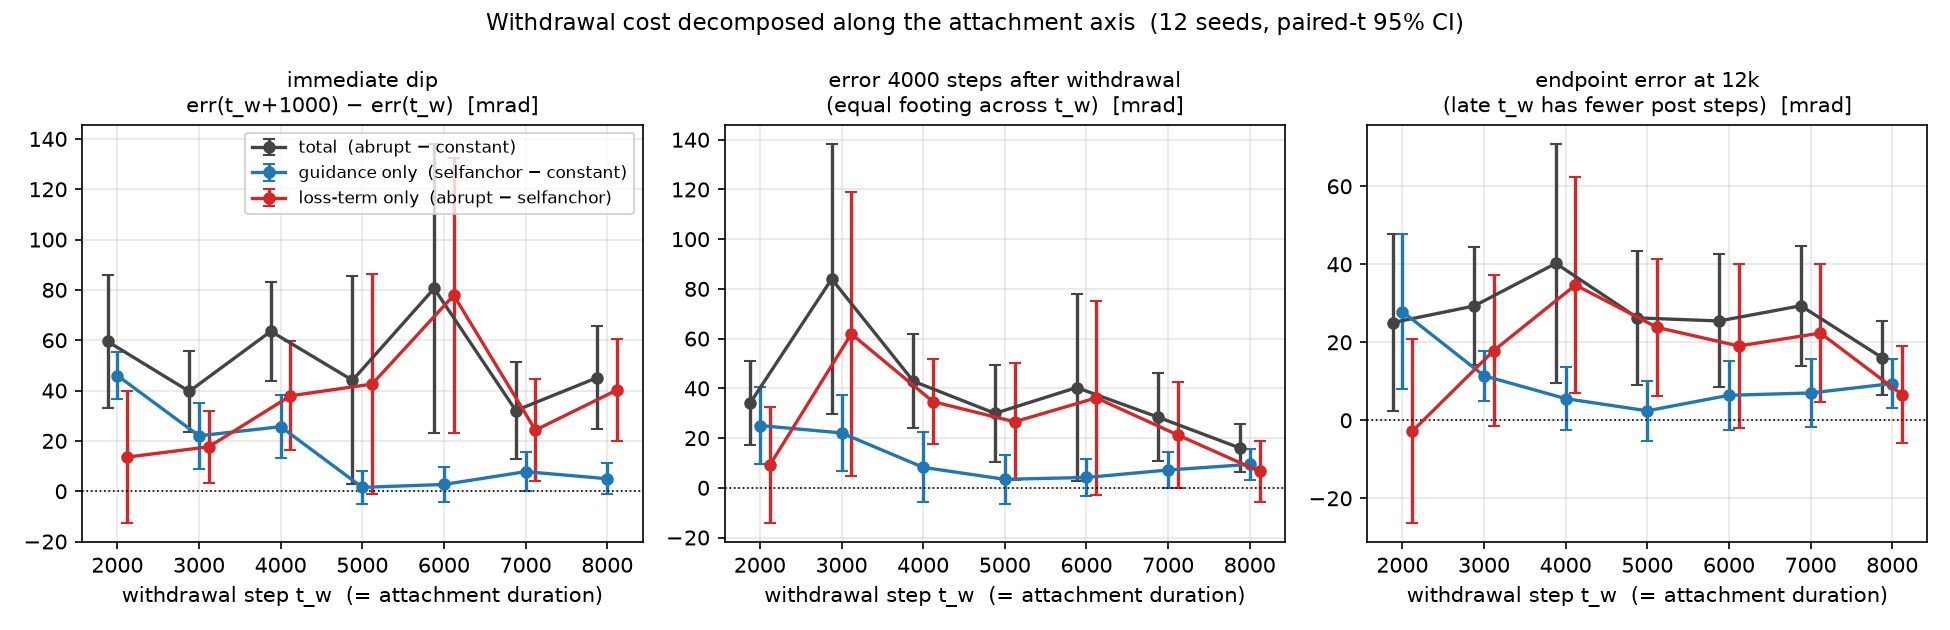
\includegraphics[width=0.84\textwidth]{figs/attachment_components_mrad.png}\\[2pt]
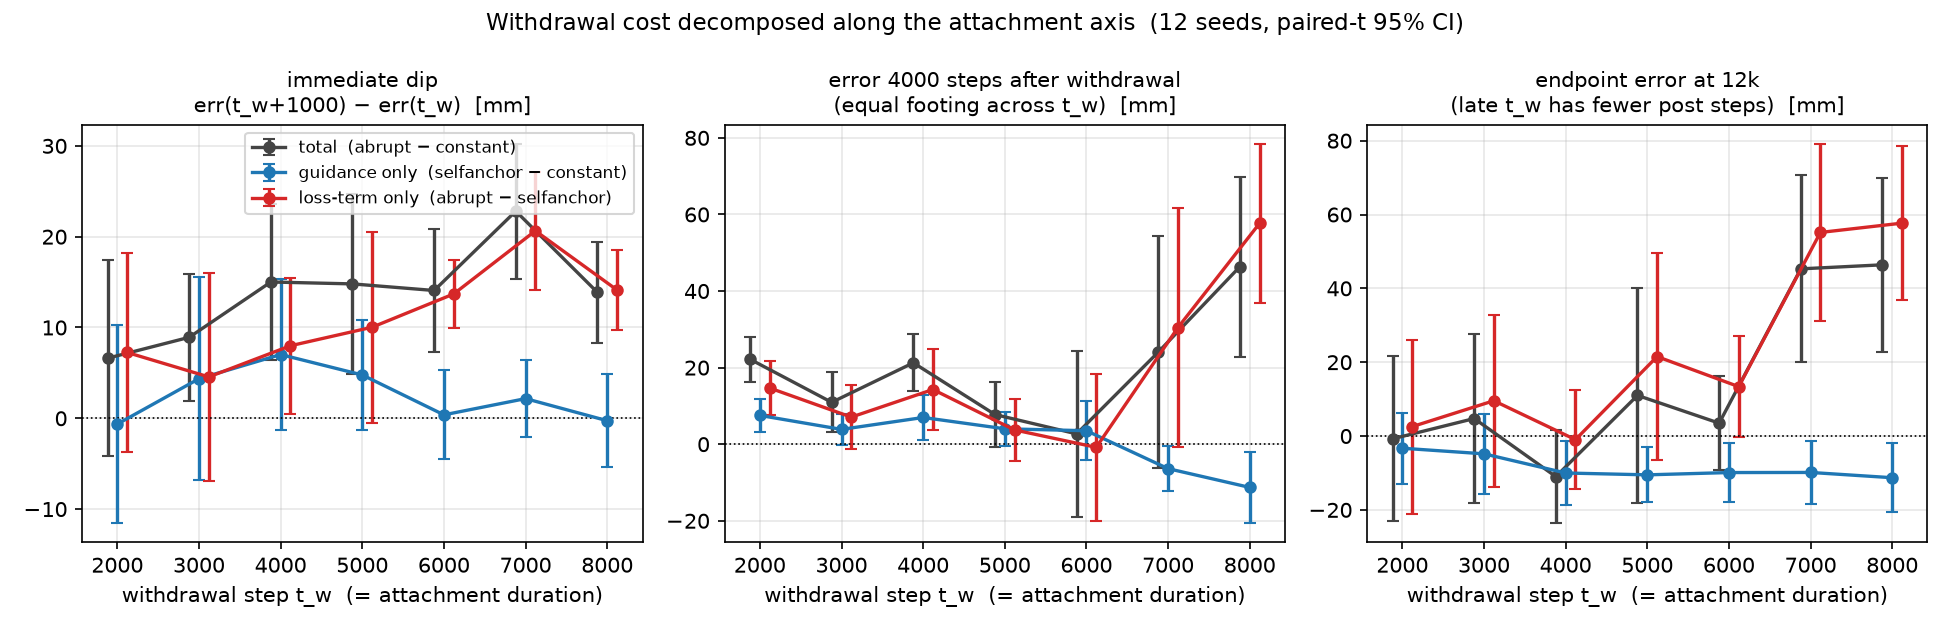
\includegraphics[width=0.84\textwidth]{figs/attachment_components_mm.png}
\caption{Teacher-withdrawal components against attachment duration on myoElbow
(top, mrad) and myoFinger (bottom, mm): total (black), teacher only (blue), loss
term only (red); $n=12$, paired-$t$ 95\% intervals. Panels: immediate dip, error
4{,}000 steps after withdrawal, endpoint.}
\label{fig:sweep}
\end{figure*}

\begin{table}[!t]
\caption{Both withdrawal decompositions on myoElbow, withdrawn at 8000, scored
at 100{,}000, $n=12$; the 12k column repeats the values these same runs give at
their 12k checkpoint. Positive means withdrawal made the arm worse. Body-model
arm means at 100k: keep 25.78, soft 33.18, purge 31.12, matched 30.84.}
\label{tab:w100k}
\centering\footnotesize
\setlength{\tabcolsep}{2pt}
\begin{tabular}{@{}lrr@{}}
\toprule
 & 12k & 100k \\
\midrule
\multicolumn{3}{@{}l}{\emph{body model}}\\
\texttt{purge}$-$\texttt{keep}   & $+7.17$ & $+5.34\ [-3.14, +13.81]$ \\
\texttt{soft}$-$\texttt{keep}    & $+2.09$ & $\mathbf{+7.40}\ [+2.72, +12.08]$ \\
\texttt{matched}$-$\texttt{keep} & $\mathbf{+22.11}$ & $+5.05\ [-0.98, +11.08]$ \\
\texttt{soft}$-$\texttt{matched} & $\mathbf{-20.02}$ & $+2.35\ [-4.42, +9.11]$ \\
\texttt{purge}$-$\texttt{matched} & $-14.94$ & $+0.28\ [-8.15, +8.72]$ \\
\midrule
\multicolumn{3}{@{}l}{\emph{teacher}}\\
\texttt{abrupt}$-$\texttt{constant}     & $\mathbf{+16.00}$ & $\mathbf{+10.29}\ [+3.96, +16.62]$ \\
\texttt{selfanchor}$-$\texttt{constant} & $\mathbf{+9.42}$  & $\mathbf{+8.16}\ [+2.17, +14.14]$ \\
\texttt{abrupt}$-$\texttt{selfanchor}   & $+6.59$ & $+2.13\ [-3.64, +7.90]$ \\
\bottomrule
\end{tabular}
\end{table}
\textbf{At one withdrawal point.} Table~\ref{tab:decomp} decomposes the
withdrawal cost at $t_w=8000$. The immediate dip is the loss term: 89\% of it
on the elbow and all of it on the finger. On the elbow a genuine cost of losing
the teacher appears only at the endpoint (\ci{+9.42}{+3.13}{+15.70}), so
short-term and long-term attributions are opposite within one experiment. On
the finger there is none: swapping in the zero-information anchor beats keeping
the teacher (\ci{-11.29}{-20.65}{-1.93}), \texttt{selfanchor} is the only arm
in which all twelve seeds recover their pre-withdrawal error, and the teacher is
not helping at 12k ($\text{constant}-\text{none}$ \ci{+5.17}{-26.49}{+36.82}).
The \texttt{randanchor} arm is worse than \texttt{selfanchor} on both bodies
and both metrics, so the anchor's content matters: \texttt{selfanchor} is not
``any loss term'' but a zero-information one pointing in the right direction,
which is what a control for the loss term should be. The finger \texttt{abrupt}
arm does not dip and recover: it is at 131~mm one thousand steps after
withdrawal and 169 at 12k, with the entropy temperature unchanged across arms,
a drift of the policy under the reward gradient once the regulariser is
removed.

\textbf{Along the attachment axis.} The hypothesis predicts that the cost of
losing the teacher grows with how long it was attached. We withdrew at every
1{,}000 steps from 2{,}000 to 8{,}000, running \texttt{abrupt} and
\texttt{selfanchor} at each point with \texttt{constant} and \texttt{none}
shared (Table~\ref{tab:sweep}, Fig.~\ref{fig:sweep}). On myoElbow the teacher
component of the dip is significant at $t_w\le4000$ and null from 5{,}000 on;
the per-seed slope is \ci{-6.23}{-7.79}{-4.68}~mrad per 1{,}000 attached steps
and no seed deviates from the downward direction. The component tracks how much
the teacher is contributing at that moment ($\text{constant}-\text{none}$ at
each $t_w$: $-86$, $-90$, $-66$, $-55$, $-24$, $-25$, $-44$), not an
accumulated reliance. The loss-term component does not decay (slope
\ci{+4.76}{-0.13}{+9.65}) and is large and noisy at $t_w=6000$, where several
\texttt{abrupt} seeds collapse; we claim that it does not decay, not that it
grows. On myoFinger the total dip \emph{does} grow with attachment (slope
\ci{+1.74}{+0.25}{+3.22}~mm per 1{,}000 steps), the textbook signature of the
hypothesis; but the teacher component is null at every $t_w$ (slope
\ci{-0.35}{-1.46}{+0.75}) and the growth is entirely the loss-term component
(slope \ci{+2.09}{+0.46}{+3.72}). At post-4k the teacher component turns
negative late ($t_w=7000$: $-6.39^*$; $8000$: $-11.29^*$; slope
\ci{-2.87}{-4.27}{-1.47}) and the loss-term slope is \ci{+5.74}{+1.49}{+9.98}:
the longer the teacher was attached, the better off the student is for having
swapped it out, and the worse for having had the term deleted. A study
measuring the total drop alone would report the hypothesis confirmed on this
body.

\textbf{At a converged budget.} The lower half of Table~\ref{tab:w100k} and the
right panel of Fig.~\ref{fig:w100k} run the elbow decomposition at $t_w=8000$ to 100{,}000 steps. Unlike the body
model's, the teacher's cost is not a transient, and by 100k it is almost
entirely the information component: $\text{abrupt}-\text{constant}$ is
\ci{+10.29}{+3.96}{+16.62}, down from $+16.00$ at 12k but still detected; of
it, losing the teacher's information accounts for \ci{+8.16}{+2.17}{+14.14}
($\text{selfanchor}-\text{constant}$), while the loss-term component,
\ci{+2.13}{-3.64}{+7.90} ($\text{abrupt}-\text{selfanchor}$), is no longer
detected. What survives training is the loss of a competent teacher, not the
optimisation event of deleting the term, and it is still not a cost that grew
with attachment.

\subsection{When guidance replaces the learner's own signal}
\label{sec:replace}

\begin{table*}[!t]
\caption{Replacing regime, myoElbow. Dip in mrad at each $t_w$, and per-seed
slopes of the post-4k and endpoint metrics. Endpoints: constant 27.86; abrupt
107.7, 133.0, 168.2, 180.8; selfanchor 45.9, 59.8, 110.8, 86.7.}
\label{tab:replace}
\centering\small
\setlength{\tabcolsep}{7pt}
\begin{tabular}{@{}lcccc cc@{}}
\toprule
 & 2k & 4k & 6k & 8k & slope post-4k & slope endpoint\\
\midrule
selfanchor $-$ constant & $58.7^*$ & $104.7^*$ & $109.4^*$ & $67.2^*$ & $+5.77$ $[+1.30,\,+10.25]^*$ & $+8.66$ $[+2.99,\,+14.33]^*$\\
gateon $-$ constant     & $59.1^*$ & $105.4^*$ & $110.2^*$ & $64.1^*$ & $+5.90$ $[+0.26,\,+11.54]^*$ & $+8.82$ $[+2.58,\,+15.06]^*$\\
\textbf{selfanchor $-$ gateon} & $\mathbf{-0.4}$ & $\mathbf{-0.8}$ & $\mathbf{-0.8}$ & $\mathbf{+3.0}$ & $-0.13$ $[-3.44,\,+3.19]$ & $-0.15$ $[-5.25,\,+4.95]$\\
abrupt $-$ selfanchor   & $54.4^*$ & $86.5^*$ & $58.6^*$ & $76.4^*$ & $+4.32$ $[-4.60,\,+13.24]$ & $+4.06$ $[-1.82,\,+9.95]$\\
abrupt $-$ constant     & $113.1^*$ & $191.2^*$ & $168.0^*$ & $143.6^*$ & $+10.10$ $[+0.52,\,+19.68]^*$ & $+12.72$ $[+6.47,\,+18.98]^*$\\
\bottomrule
\end{tabular}
\end{table*}
The additive coach is the wrong model of physical guidance, which substitutes
for the learner's own error correction rather than supplementing it. The
replacing regime is the right one, and it is also what reward-free distillation
does in current humanoid pipelines \cite{rudin2022}. We ran it on myoElbow at
$t_w\in\{2000,4000,6000,8000\}$ with \texttt{constant}, \texttt{abrupt},
\texttt{selfanchor} and \texttt{gateon} (Table~\ref{tab:replace}). Without the
\texttt{gateon} arm the first row confirms the hypothesis: the cost of losing
the teacher is large at every $t_w$ and grows with attachment (post-4k slope
\ci{+5.77}{+1.30}{+10.25}; endpoint slope \ci{+8.66}{+2.99}{+14.33}), an order
of magnitude above the additive regime at late $t_w$. With it the confirmation
dissolves. Keeping the real teacher while switching on the student's own
gradient produces the same collapse, seed by seed:
$\text{selfanchor}-\text{gateon}$ is within 3.1~mrad at every $t_w$, with
intervals as narrow as $[-2.5,+1.7]$, and no significant slope on any metric.
What grows with attachment is the cost of first activating the learner's own
policy gradient after a cloning-only phase, the known collapse when a
behaviour-cloned policy is fine-tuned by off-policy reinforcement
\cite{nair2020,uchendu2023,zhang2023}, and it is unrelated to the teacher.
After a cloning-only phase the student's snapshot \emph{is} the teacher, so
\texttt{selfanchor} cannot price the teacher's information in this regime;
\texttt{gateon} can, and finds none. The pure-distillation \texttt{constant}
arm ends at 27.86~mrad, better than the additive constant (39.13), and
\texttt{abrupt} in this regime, plain SAC after $t_w$, recovers in 0 of 12
seeds at $t_w=4000$ and 6{,}000, ending at 133 and 168~mrad, worse than a
student that never had a teacher (70.73).

\section{Discussion}

\textbf{What dependence would have to look like.} The self-anchor control
makes the notion measurable: dependence is the part of the withdrawal cost that
survives replacing the teacher by a zero-information stand-in, and the guidance
hypothesis predicts that this part grows with attachment. On two bodies, seven
durations, and two regimes, it never does. In the additive regime it tracks the
teacher's current contribution and fades as the learner becomes competent; on
the finger, where the teacher contributes little at any time, it is null
throughout and swapping the teacher out is better than keeping it. In the
replacing regime the growing cost is real but belongs to the learner's own
machinery, an actor that has never been moved by its critic, not to the
teacher. What does persist on the elbow to a converged budget is about 8~mrad
of genuinely lost teacher information, with the loss-term shock gone; that is
the cost of no longer having a competent teacher, and it did not grow with how
long the teacher was attached. The hypothesis' mechanism, that guidance
prevents the learner from practising its own error correction
\cite{schmidt1992}, has a visible shadow here: a cloning-only actor pays for
not having practised when its own gradient is switched on, and pays more the
longer it went without. But the human prediction is about the guidance being
missed, and that is what we do not find. The zero-information anchor has a
natural human analogue, guidance that is present but carries no information
about the target, and the question is now a precise one.

\textbf{Guidance is only as good as its teacher.} On the acquisition limb the
coach does what the hypothesis says on both bodies through 8k. What happens
after that is body-dependent in a way the hypothesis does not predict but does
explain. On the elbow the teacher is competent and the student, held near it,
plateaus near it, keeping a small advantage over model-free learning at
convergence. On the finger the teacher is within 3.2~mm of doing nothing; a
student held near it is held near a policy that does not move, by 40k it is
worse than no aid, and at convergence it is worse than a student held near a
random teacher. A constant pull toward a poor target is a ceiling, not a prior,
and a body model that on its own beats model-free learning by 40~mm cannot pull
a student out of it.

\textbf{The body model helps where the body is hard.} Internal-model theory
would have a learned body model help most where the body is hardest to control
without one, and that is the direction the two bodies take: on the one-joint
elbow a model-free learner closes the gap by 100k and the model's benefit is a
transient of the first 12k; on the four-joint finger it is present at
convergence and at nearly every checkpoint before it. On the elbow what the
model is worth at 8k is carried by the imagined transitions already stored, and
deleting them costs 20~mrad in the window after the cut, which the original
protocol could not see because it deleted them and doubled the real-data signal
in the same step; by 100k that cost is gone and the arm that kept a stale buffer
is the worst of the four. The body model's value on this body is front-loaded
and temporary, consistent with its endpoint advantage being a transient of the
same window. The caveats are that the elbow's generalisation test is weak, that
two bodies are an ordering and not a law, and that the prior arm is handed the
analytic reward at imagined states, which no biological reading can take for
granted.

\textbf{Measurement.} Each of the three results needed a measurement the
literature does not usually make. An endpoint fixed in advance and not verified
as an asymptote landed inside a transient on both bodies; budgets of the order
of 12k are common in muscle control, and the remedy is not a larger number but
a check that the arms have stopped moving. A withdrawal that changes two things
at once cannot be read as the cost of the thing withdrawn; the body-model side
needed a matched-replay arm, the teacher side a self-anchor, and a cloning-only
pipeline a \texttt{gateon} arm as well, since a distillation learner with no
reward term \cite{rudin2022} freezes when its coefficient is zeroed and the
swap is the only withdrawal that means anything. Fading schedules deserve the
same decomposition: a taper spreads the loss-term deletion over time and may be
reducing the shock rather than the dependence.

\section{Limitations}
\label{sec:limits}
The study is single-task reach, simulation only, on deterministic and fully
observed bodies, conditions that favour a frozen forward model. Two bodies are
analysed; myoElbow has one degree of freedom, so its twenty held-out targets
interpolate between eight training targets and its generalisation test is weak.
One teacher per body: the finger teacher as captured scores 169.1~mm against a
zero-activation no-op referent of 172.3, an unreplicated 3.2~mm not
distinguishable from doing nothing, so every finger result for the guidance
route is a result about distilling toward a near-no-op target. $n=12$ seeds
throughout. The two routes are not matched in what they consume: the prior arm
holds the analytic reward at imagined states, and the Dyna arms train on 64 real
and 64 imagined transitions where model-free arms train on 128 real, so equal
update-to-data is not equal real-data signal; the \texttt{matched} arm controls
this at withdrawal, not during training. The body-model withdrawal result is an
elbow result, and the converged decompositions were run on the elbow only. One
withdrawal shape (a step, no taper); seven attachment points give a short trend
test, and the loss-term slope is marginal on the elbow and non-monotone on the
finger, so we claim that it does not decay, not that it grows monotonically. In
the replacing regime \texttt{selfanchor} coincides with the teacher by
construction, and that regime was run on the elbow only. Contrasts were chosen
during the study and not pre-registered. No physical robot is involved, and the
humanoid pipelines that motivate the teacher experiments use on-policy learners
whose transition costs may differ in size, though not, we expect, in kind.

\section{Conclusion}
Two routes to a motor prior were compared under one backbone on two
musculoskeletal bodies, to a converged budget, with each route given the
adversarial control the other has and with the withdrawal of each made
single-factor. The body model helps where the body is hard: transient on the
elbow, stable on the finger. Guidance is only as good as its teacher: a small
lasting advantage where the teacher is competent, a ceiling below model-free
learning where it barely moves. And withdrawing either prior costs no
dependence: the body model's cost is a transient the standard protocol misses,
and the teacher's, once a zero-information stand-in separates the loss term
from the teacher, never grows with attachment and ends as the loss of a
competent teacher. An early endpoint reversed the first two verdicts; matching
data budgets changed none.

\bibliographystyle{IEEEtran}
\bibliography{refs}

\end{document}
